\documentclass{article}
\usepackage[utf8]{inputenc}

\usepackage[paperwidth=8.5in, paperheight=11in, top=1in, bottom=.5in, left=.5in, right=.5in]{geometry}
\usepackage{fancyhdr, graphicx,tikz,amsmath,multicol,paracol}
\usepackage[inline]{enumitem}


\pagestyle{fancy}
\lhead{\large{\textbf{Module 4: Polynomial and Rational Functions - Readiness Assurance Test}}}
\chead{}
\rhead{}
\lfoot{}
\cfoot{}
%\rfoot{\thepage/\pageref{LastPage} }
\setlength{\headheight}{14pt} %added in bc warning

%%% LIST ANSWER KEY HERE

% 1 A
% 2 C
% 3 A
% 4 A
% 5 D
% 6 A
% 7 B
% 8 A
% 9 C
% 10 D


\begin{document}


\begin{enumerate}

  
 %Find the degree and leading coefficient of a polynomial.
 \item Find the degree and leading coefficient of the polynomial \(4x^3+3x^2-5x-8\).


  \begin{enumerate}
  \item degree \(3\), leading coefficient \(4\)  %correct 
  \item degree \(4\), leading coefficient \(3\)
  \item degree \(3\), leading coefficient \(-8\)
  \item degree \(8\), leading coefficient \(4\)
  \end{enumerate}
  
 %Find the intercepts of a line.
\item Find the intercepts of the line \(y=4x-8\).
  \begin{enumerate}  
  \item \(x\text{-}\)intercept \((0,-8)\), \(y\text{-}\)intercept \((2,0)\) 
  \item \(x\text{-}\)intercept \((0,2)\), \(y\text{-}\)intercept \((-8,0)\)
  \item \(x\text{-}\)intercept \((2,0)\), \(y\text{-}\)intercept \((0,-8)\) %correct
  \item \(x\text{-}\)intercept \((0,0)\), \(y\text{-}\)intercept \((0,-8)\) 
  \end{enumerate}

\item Find the equation of the line passing through the points \((4,5)\) and \((2,8)\).
 %Find the equation of a line passing through two points

  \begin{enumerate}
  \begin{multicols}{4}
  \item \(y=-\frac{3}{2}x+11)\) %correct
  \item \(y=-\frac{3}{2}x+5)\)
  \item \(y=\frac{3}{2}x+11\)
  \item \(y=-\frac{2}{3}x+8)\)
  \end{multicols}
  \end{enumerate}

  \item Factor the polynomial \(9x^4+3x^3-12x^2\) completely.
 %Factor quadratics and polynomials

  \begin{enumerate}
  \item \(3x^2(x-1)(3x+4)\) %correct
  \item \(3x^2(x+1)(3x-4)\)
  \item \(3x^2(3x^2+x-4)\)
  \item \(3x^2(3x-1)(x+4)\)
  \end{enumerate}

  \item Solve the quadratic equation \(x^{2}-2x+5=0\). 
  %Solve the quadratic with complex roots.

  \begin{enumerate}
  \begin{multicols}{4}
  \item \(1\pm 4i\)
  \item \(-1, 3\)
  \item \(2\pm 2i\)
  \item \(1\pm 2i\) %correct
  \end{multicols}
  \end{enumerate}

  \item Simplify the rational expression \(\dfrac{x^2+x-42}{x^2-36}\).
 %simplify rational expression

  \begin{enumerate}
  \begin{multicols}{4}
  \item \(\dfrac{x+7}{x+6}\) %correct
  \item \(\dfrac{x-7}{x-6}\)
  \item \(\dfrac{x+7}{x-6}\)
  \item \(\dfrac{x-6}{x+6}\)
  \end{multicols}
  \end{enumerate}

  \item Let \(f(x)=\dfrac{x^2-1}{x+3}\). Find \(f(-4)\).
 %Evaluate a function from an equation.

  \begin{enumerate}
  \begin{multicols}{4}
  \item \(\dfrac{15}{7}\) 
  \item \(-15\) %correct
  \item \(15\)
  \item \(-\dfrac{15}{7}\)
  \end{multicols}
  \end{enumerate}

  \item On what interval is the graph decreasing?
 %find where a graph is increasing and decreasing.
 
     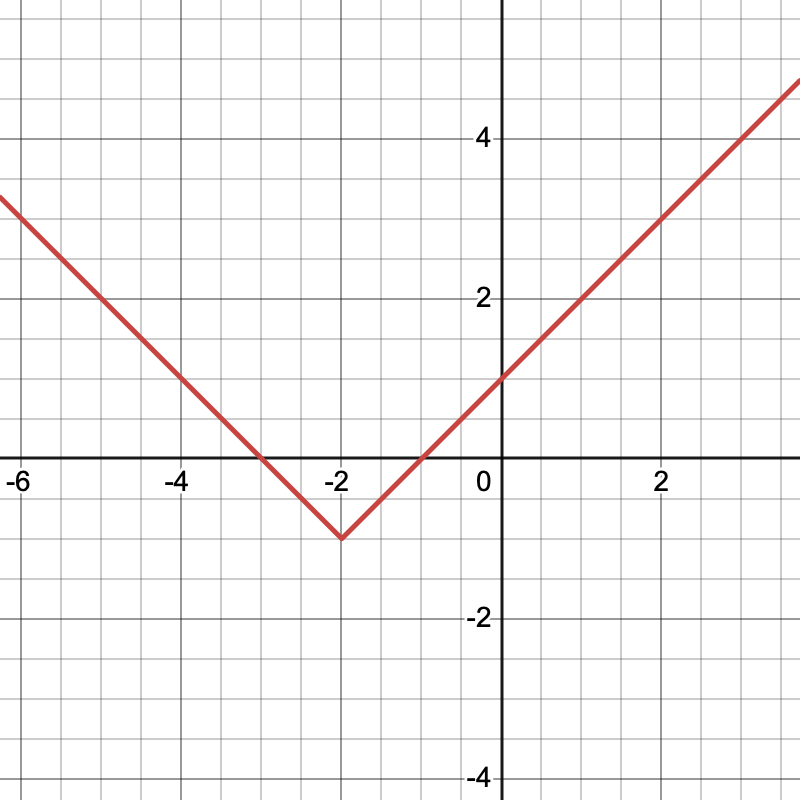
\includegraphics[width=0.25\linewidth]{desmos-graph-3.png}

  \begin{enumerate}
  \begin{multicols}{4}
  \item \((-\infty, -2)\) %correct
  \item \((-2,\infty)\)
  \item \((-\infty, -1)\)
  \item \((-1,\infty)\)
  \end{multicols}
  \end{enumerate}

   \item Which of the following graphs represents a polynomial?
%determine if a graph is a polynomial
  \begin{enumerate}
  \begin{multicols}{2}
  \item  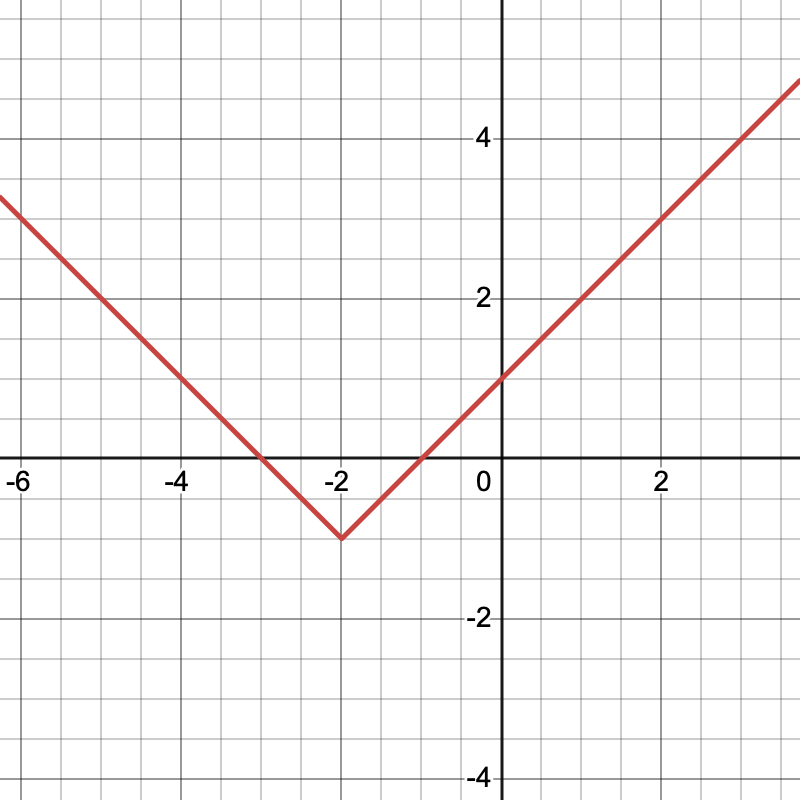
\includegraphics[width=0.25\linewidth]{desmos-graph-3.png} 
   \item  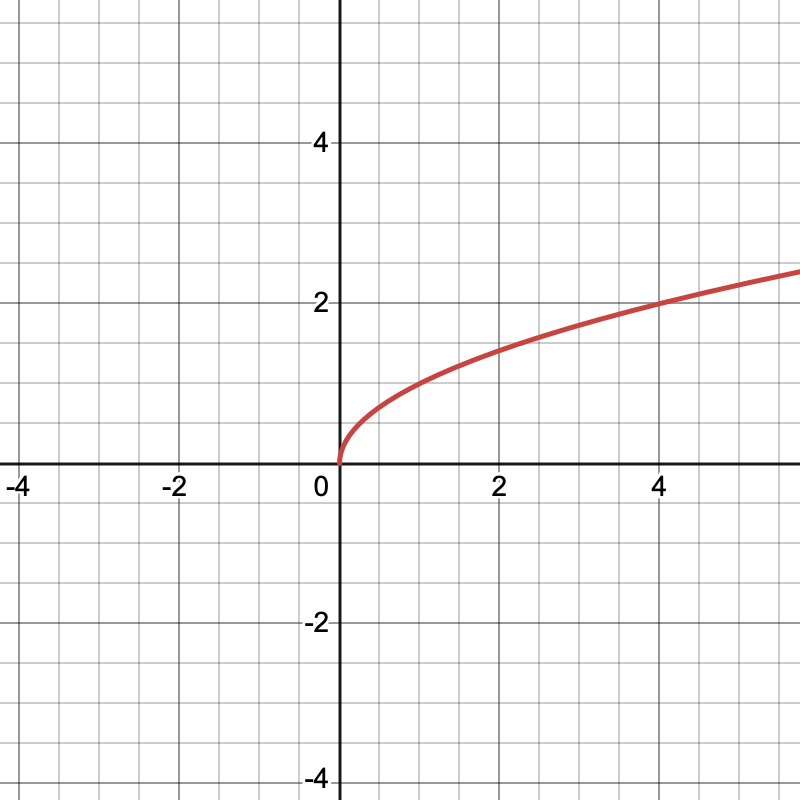
\includegraphics[width=0.25\linewidth]{desmos-graph-4.png} 
  \item  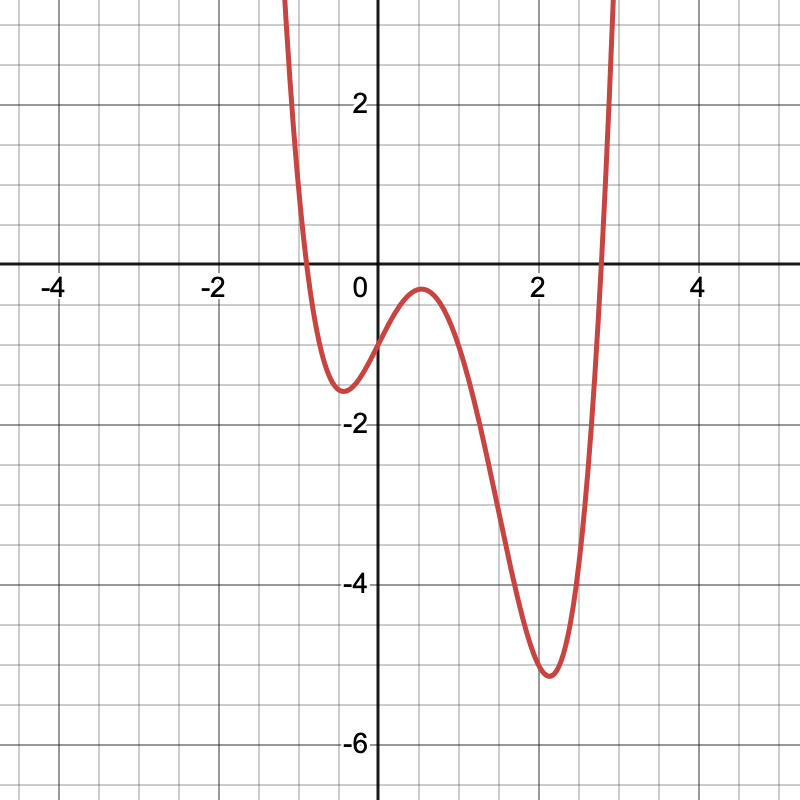
\includegraphics[width=0.25\linewidth]{desmos-graph-6.png}  %correct
   \item  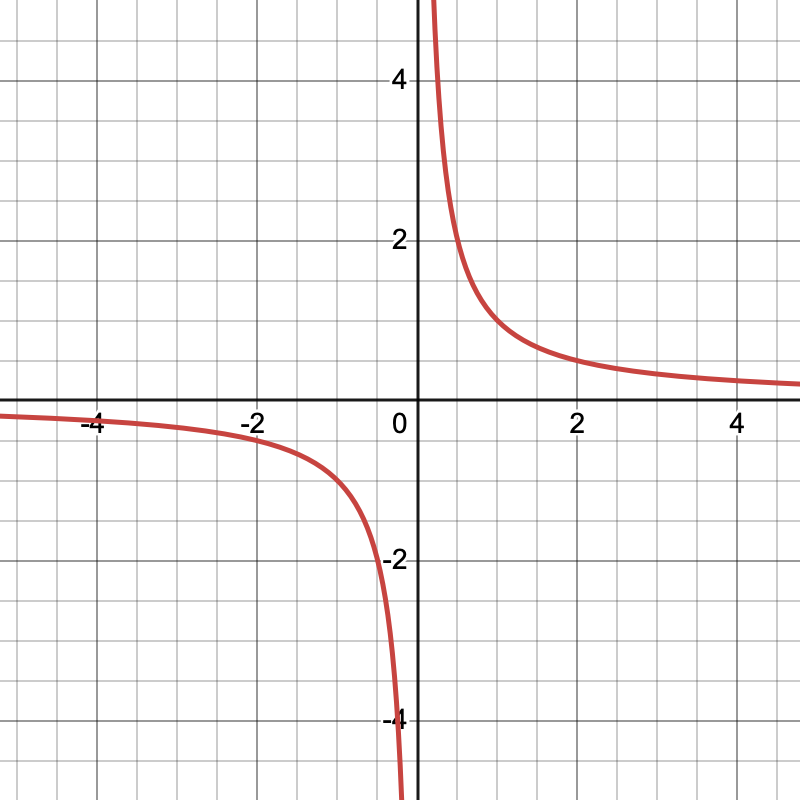
\includegraphics[width=0.25\linewidth]{desmos-graph-5.png}
  \end{multicols}
  \end{enumerate}

 %Find the intercepts from a graph
\item Find the intercepts of the function graphed below.

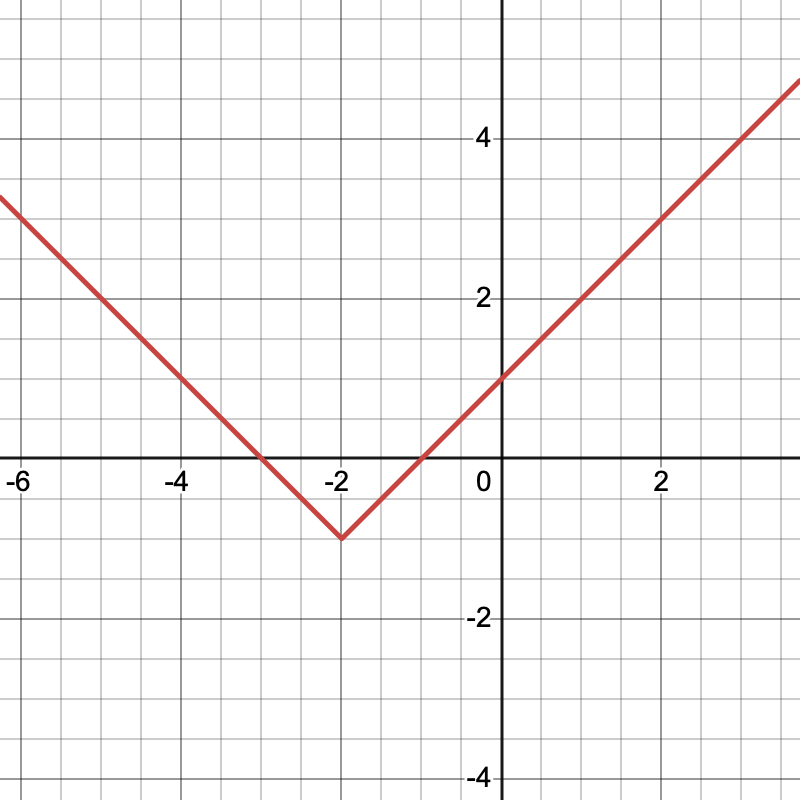
\includegraphics[width=0.25\linewidth]{desmos-graph-3.png} 
  \begin{enumerate}  
  \item \(x\text{-}\)intercept \((-2,0)\), \(y\text{-}\)intercept \((0,-1)\) 
  \item \(x\text{-}\)intercepts \((0,-3)\) and \((0,-1)\), \(y\text{-}\)intercept \((1,0)\) 
  \item \(x\text{-}\)intercept \((1,0)\), \(y\text{-}\)intercepts \((-3,0)\) and \((-1,0)\)
  \item \(x\text{-}\)intercepts \((-3,0)\) and \((-1,0)\), \(y\text{-}\)intercept \((0,1)\)  %correct
  \end{enumerate}



\end{enumerate}


\end{document}
